\section{Existing Index Structures}
\label{sec:structures}

Many index structures have been developed throughout the past forty years, such as quadtrees in the early 1970s \cite{quadtree} and splay quadtrees in 2012 \cite{splay-quadtree}. New structures are often based on older index structures, either by modifying an existing structure or combining two different structures in some way. Figure \ref{fig:structure-taxonomy} in Appendix \ref{chap:supp-material} shows a \textit{taxonomy} of index structures. This section describes some of the widely used index structures, their limitations (with respect to the challenges discussed in Section \ref{sec:challenges}) and why this led onto the development of new structures.

\subsection{Basic Structures}
\label{sec:basic-structures}

\textbf{Sequential scan} refers to the brute-force approach of searching a data set. You simply store the dataset in a linear data structure (e.g. a list) and iterate through each data item until the desired point is found. This means searching is an $O(n)$ operation. Using a standard array, insertion is $O(1)$ if new points are inserted at the end of the array and deletion is $O(n)$. There is little memory overhead for this approach, but search times will be very long if there are large number of points. Nevertheless, if the number of data items is small, a more complex index structure may not be needed.

Search trees order data items in a hierarchical fashion to make search faster \cite{introduction-to-algorithms}. The \textbf{binary search tree}, for one-dimensional data, is one of the first of these trees and is the basis of many index structures \cite{introduction-to-algorithms}. Each node stores a \textit{key}, which is a total orderable element. Each non-leaf node has at most two children, where the left child's key is less than its parent's and the right child's key is greater than or equal to its parent's. This property is referred to as \textit{key order} \cite{rst}. When inserting or deleting new points, the key order invariant must be maintained. Maintaining this invariant can be done in $O(n)$ time \cite{introduction-to-algorithms}, making insertion and deletion $O(n)$.

A point query is equivalent to checking if a certain key is stored in the tree. In the best case, we get running time $O(\log_2 n)$ for the query, because $\log_2 n$ is the \textit{minimum} height of the tree. However, this performance is not guaranteed. Skewed or sorted data may result in taller trees, where there are many nodes with only left or only right children. This makes the binary tree \textit{unbalanced} (height greater than $\log_2 n$). If balance is not guaranteed, the running time of a point query is $O(n)$ in the worst case, which is no better than a sequential search.

\textbf{Balanced search trees} re-order the nodes to maintain balance (logarithmic height) when a node is inserted, updated or deleted, regardless of data skew. These operations cause dynamic index structure operations to become slower, but allow for faster queries.  Maintaining balance is one-dimensional trees is well-solved, but much more difficult for multi-dimensional trees. Many one-dimensional balanced search trees exist, including red-black trees, AVL trees, splay trees and treaps \cite{introduction-to-algorithms}.

\subsection{Recursive Partitioning of Data Space}
\label{sec:recursive-partition-structures}

Index structures which decompose the data space into sub-spaces recursively are popular \cite{md-structures-samet}. The decomposed space is represented as a search tree. If $R$ is some $d$-dimensional data space, then $R_1,...,R_x$ are the decomposed sub-spaces (often disjoint) of $R$ . $R$ becomes the root node and $R_1,...,R_x$ become the children of $R$ in the tree representation. Each of those sub-spaces may then be decomposed in a similar way, increasing the depth of the tree.

This is useful because it allows large amounts of the data space to be discarded from consideration at once. Consider a point query with a point $p$. $p \in R$ since R is the entire data space. Assuming a disjoint decomposition was used, if $p \in R_1$ then $p \not\in R_2,...,R_x$. Since it is known that $p$ is only in $R_1$, only $R_1$'s children need to be checked -- the rest of the tree can be \textit{ignored}.

\subsubsection{Quadtrees}

A quadtree is one of the earliest index structures based on disjoint recursive decomposition of space, specifically created for two-dimensional space \cite{original-quadtree}. \textbf{Octrees} are a generalisation of quadtrees to $d \geq 2$ dimensions. Throughout the past forty years, many variations of the quadtree have been produced. Hanan Samet produced a survey describing many uses and variants of this data structure in  \cite{quadtree} and twenty years later, there are even more variants. Several variants are discussed in this review, but it is beyond the scope of this report to list all of them.

PR quadtrees are a commonly used quadtree which partition the data space into $2^d$ uniformly sized sub-spaces. This means quadtree nodes have up to $2^d$ children. This process can be repeated recursively to produce a grid with increasingly smaller cells. Figure \ref{fig:quadtree-clustered} shows an example of a PR quadtree decomposition of some data. Notice how the underlying data space is decomposed in the same way, regardless of where the points in the dataset are in the space.

An advantage of PR quadtrees is that there is no overlap between the spatial regions represented by two sibling nodes. This greatly simplifies \texttt{insert}, \texttt{update} and \texttt{delete} operations. However, they do not perform well with \textbf{non-uniform} data. So if there are clusters or skews of data, then there will be many empty (or near empty) quadtree nodes/regions (see Figure \ref{fig:quadtree-clustered}). These empty, unnecessary nodes may be searched during queries, reducing performance.

\begin{figure}
	\begin{center}
		\begin{subfloat}[PR Quadtree\label{fig:quadtree-clustered}]{%
			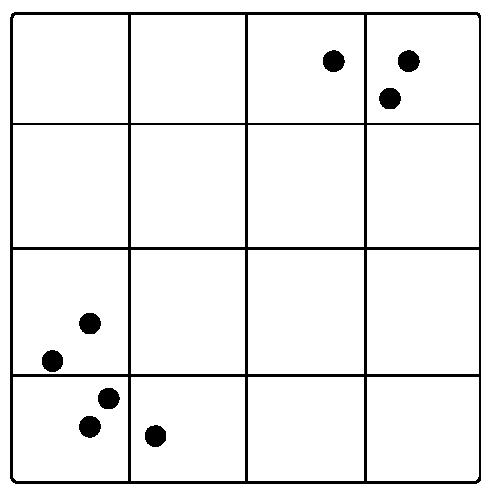
\includegraphics[scale=0.4]{figures/quadtree_clustered.pdf}
		}
		\end{subfloat}~~~~~
		\begin{subfloat}[Point $kd$-Tree\label{fig:kdtree-clustered}]{%
			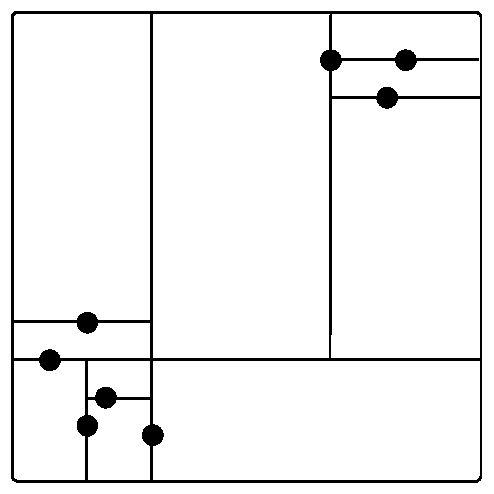
\includegraphics[scale=0.4]{figures/kdtree_clustered.pdf}
		}
		\end{subfloat}~~~~~
		\begin{subfloat}[Binary Space Partition\label{fig:bsp}]{%
			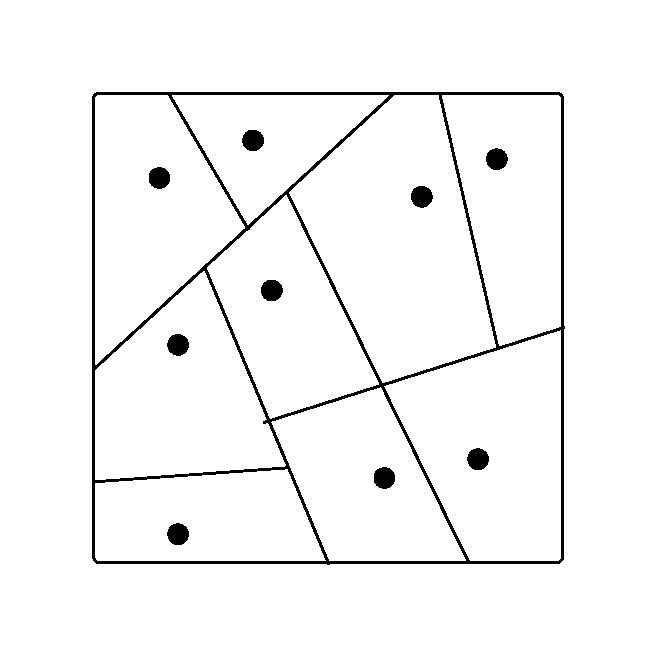
\includegraphics[scale=0.4]{figures/bsp_tree.pdf}
		}
		\end{subfloat}
	\end{center}

	\caption{Spatial Decompositions Created With Various Tree-Based Index Structures}
	\label{fig:tree-based-decomposition}
\end{figure}

\subsubsection{$kd$-trees}

$kd$-trees are similar to quadtrees in that the data space is partitioned into disjoint regions \cite{kd-tree}. Unlike quadtrees, nodes have at most two children regardless of dimensionality. Each node in the tree splits the current region of data space into two sub-regions along a single dimension $i$. These sub-regions are represented as two nodes, whose parent is the node representing the original region. A \textit{pivot} value $p$ is chosen for $i$. The left and right children contain all the data items whose $i$th value is less than $p$ and greater than or equal to $p$ respectively. How a $kd$-tree is built depends on how $i$ and $p$ are chosen, so there are many variations of this structure. There are two major types of $kd$-tree -- point and bucket \cite{md-structures-samet}. Point $kd$-trees store a single point in each node of the tree, meaning there are always $n$ nodes. Bucket $kd$-trees only store points in the leaves, which can contain multiple points.

Unlike the PR quadtree, $kd$-trees can produce non-uniform partitions, making the structure better suited to skewed or clustered data. Figures \ref{fig:quadtree-clustered} and \ref{fig:kdtree-clustered} show a PR quadtree and point $kd$-tree partition of some clustered data. Notice how there are more empty regions in the quadtree than the $kd$-tree, thus having a less efficient partition of the data.

Like binary search trees, it is ideal to maintain a \textit{balanced} tree to minimise height and ensure queries can be performed quickly. Dynamically inserting or deleting points can unbalance the tree. Variants of bucket $kd$-trees have been developed to maintain a balanced tree and fast query times. Examples of such variants include the BD-tree \cite{kdtree-v-bdtree} and KDB-tree \cite{kdb-tree}.

\subsubsection{Binary Space Partitioning}

BSP (binary space partitioning) trees are a generalisation of kd-trees that use hyperplanes (lines in 2D, planes in 3D) to recursively partition the data space \cite{bsp-tree}. That is, it partitions data space $S$ into two disjoint sub-spaces $S_1$ and $S_2$. This process is repeated recursively using different hyperplanes for each split. A BSP tree decomposition is illustrated in Figure \ref{fig:bsp}.

Optimal BSP trees allow efficient point queries to be performed by discarding as many points as possible at each level of the tree (i.e. the tree has low height). Finding optimal BSP trees for a given set of data points is an $\mathbb{NP}$-complete problem \cite{bsp-np-hard}. When inserting, updating or deleting points a new optimal partitioning must be computed to minimise tree height, making dynamic operations very slow. Therefore, BSP trees are better suited for static data because an optimal tree can be \textit{pre-computed} and loaded into main memory during program initialisation.

\subsubsection{Skip Quadtree}

Despite the original quadtree structure being developed approximately forty years ago, researchers are still enhancing the index structure's performance in new ways. A relatively new data structure, the skip quadtree, is ``simple" to implement and benefits from low memory overhead \cite{skip-quadtree}. \textbf{Skip quadtrees} were developed with range queries in mind and are based on the concept of compressed quadtrees. \textbf{Compressed quadtrees} compress paths of nodes which only have a single non-empty child into a \textit{single node} \cite{compressed-quadtree}, which combats the effects of skewed data.

Skip quadtrees combine one-dimensional skip lists \cite{skip-quadtree} and compressed quadtrees to create an index structure with $O(\log n)$ point queries and $O(\epsilon^{1 - d} \log n + k)$ \textit{approximate} range queries, where $k$ is the size of the range and $\epsilon$ is the approximation factor that controls the accuracy of the range query \cite{skip-quadtree}. However, skip quadtrees may not be efficient for very datasets because they were not constructed with paging in mind.

\subsection{Bucket Methods}
\label{sec:bucket-methods}

\textbf{Bucket methods} were developed to increase I/O efficiency for large datasets that are paged in secondary memory. Such structures were designed to minimise the number of I/O operations (secondary memory accesses) required to perform queries (see Section \ref{sec:paging} for more discussion on this). These methods group points into contiguous blocks of memory called \textit{buckets}, which are the same size as a page in secondary memory. To reduce the number of I/O operations required to perform a query, bucket methods aim to fill each bucket with as many nodes as possible \cite{md-structures-samet}.

\textit{Fanout} refers to the amount of children each node have on average. Higher fanout results in a search tree with lower height, which means less nodes are accessed on average when searching for a point. Node access is particularly expensive when the tree has been paged into secondary memory, so some bucket methods aim to increase fanout (e.g. TV-tree \cite{tv-tree} and A-tree \cite{a-tree}).

There are two types of bucket methods \cite{md-structures-samet}:
\begin{itemize}
	\item \textbf{Overlapping Decomposition} -- these ensure that each bucket has a \textit{minimum} number of data items it must contain, which increases fanout and thus, search times. However, in the process of ensuring each bucket has a minimum amount of used capacity, the bounding regions of buckets in data space may begin overlapping. Overlapping regions means more nodes must be checked when performing a query, increasing search times.
	\item \textbf{Disjoint Decomposition} -- these ensure that there is \textit{no overlap} between buckets. This means less nodes need to be checked in a query, but there is no guarantee on how much each bucket is filled, potentially increasing the number of I/O operations performed
\end{itemize}

\subsubsection{B-Trees and B${}^{+}$-Trees}

The B-Tree was developed by Rudolf Bayer in 1972 and is often used for databases or file-systems \cite{ubiquitous-btree}. It is a one-dimensional search tree which allows for point queries, insertions and deletions to be performed in $O(\log n)$ time \cite{btree}. B-trees maintain key order, but allow nodes to have more than two children, making them a generalisation of binary search trees.

B${}^{+}$-trees are B-trees where only the \textit{leaves} contain the actual values of the data \cite{ubiquitous-btree}. This means all non-leaves simply contain pointers to, or the keys of, their children. B${}^{+}$-trees ensure that each bucket is at least 50\% full \cite{md-structures-samet, ubiquitous-btree}, which leads to less I/O operations. This is a very attractive property, as it can greatly speed up query times for large data sets. There have been many attempts to generalise the B-tree to a multi-dimensional setting while retaining this property. The k-d-B tree \cite{kdb-tree} and BV-tree \cite{bv-tree} are two examples of such attempts. Freeston in \cite{bv-tree} discusses how this ``apparently simple" objective has proved extremely difficult to achieve.

\subsubsection{R-Tree Family}

An R-tree can be thought of as a B${}^{+}$-tree that can handle multi-dimensional data, supporting data items that have non-zero size in data space (i.e. regions) \cite{r-tree}. This means nodes are represented using \textit{hyper-rectangles} that define the region of the data space all of the node's children are contained in. The running time for queries is $O(n)$ in the worst case, but expected performance is much higher. 

R-trees have attracted much attention from researchers. Many variants of the structure have been developed, such as R*-trees \cite{rstar-tree}, R+-trees \cite{rplus-tree}, SS-trees \cite{ss-tree}, RS-trees \cite{rs-tree} and Hilbert R-Trees \cite{hilbert-rtree}. Combinations of these variations also exist, such as SR-trees \cite{md-structures-samet} and RSR-trees \cite{rsr-tree}.

R-tree based structures use overlapping decomposition, which is a key performance issue \cite{pyramid-tree}. If you have a point contained in $m$ nodes' regions, all $m$ nodes could be searched. This severely limits the performance of R-tree based index structures with data spaces that have a \textbf{large} number of dimensions (see Section \ref{sec:curse-of-dimensionality} for more details).

\subsubsection{PK-Tree}

PK-trees (Pyramid K-instantiable trees) are a family of structures based on kd-trees that were created specifically to handle high-dimensional data \cite{pk-tree}. They are similar to bucket methods, but instead of imposing a minimum number of points per bucket, they impose a maximum. Imposing this maximum (called the $k$-instantiation value) results in a reduced amount of I/O operations \cite{md-structures-samet}. PK-trees bound the height of the tree to $O(\log n)$ for some data. Through tests on synthetic and real data, the PK-tree has been shown in greatly outperform the SR-tree and X-tree \cite{pk-tree}, especially for higher dimensions.

However, there are some caveats. In order for the PK-tree to have $O(\log n)$ height, certain constraints must be applied to the distribution of the data. Furthermore, the pagination of the index structure which minimises I/O operations depends on the value of $K$ (the number of children a node can have) and the size of the actual hard disk pages used by the operating system \cite{pk-tree}. The amount to split each dimension at each level is also configurable, so there are many parameters to tweak to achieve the proposed performance. Additionally, as discussed in Section \ref{sec:curse-of-dimensionality}, the PK tree's performance on very high dimensional data will be still be poor, because most index structures that decompose the underlying data space perform poorly when $d$ is high.

PK-trees are also complicated to implement. This problem is exacerbated by having to tweak many different parameters and be careful about what kind of data is stored in the tree. Therefore, due to their complexity and poor performance on very high dimensional spaces, PK-trees have not been widely adopted \cite{md-structures-samet}.

\subsection{Structures Tailored to High-Dimensional Data}
\label{sec:high-dimensional-structures}

Section \ref{sec:curse-of-dimensionality} discusses how higher dimensional data spaces cause index structures which perform well on low dimensional data to degenerate and provide poor performance. There have been efforts to develop index structures which still perform well in higher-dimensional space. Many different approaches have been used, such as tree-based spatial decompositions, distance-based methods, dimension reduction and non-hierarchical, sequential methods. Some of the more influential data structures from the literature have been identified and are described here.

\subsubsection{X-Tree}

R-tree based index structures often struggle to provide efficient queries in high-dimensional space, because the hyper-rectangles or spheres tend to overlap more \cite{pyramid-tree}. X-trees \cite{x-tree} try to reduce overlap by extending the capacity of nodes/buckets if creating a new node would result in an overlap (these are called supernodes). X-trees outperform most R-tree variants \cite{x-tree}. However, Berchtold et al. show in  \cite{pyramid-tree} show the structure still degenerates at higher dimensions ($d \geq 10$) \cite{pyramid-tree}.

\subsubsection{Distance-Based Methods}

When there are a large number of dimensions, determining which dimensions are actually relevant for searching can be difficult. In these cases, \textit{distance-based methods} may be useful. They use the similarity (distance in data space) between each pair of points to deduce more information about the relationships in the data and provide faster search \cite{md-structures-samet}. There are two major types: \textit{pivot-based}, which choose a subset of all points in the dataset to base distance measurements on, and \textit{cluster-based}, which partition the dataset's points into spatial regions called clusters that are used to compute distances \cite{md-structures-samet}. A notable distance-based index structure is the M-tree, which combines R-trees with distance-based techniques to perform high dimensional search with dynamic datasets \cite{m-tree}.

\subsubsection{Dimension Reduction}

One method of mitigating the effects of the curse of dimensionality is reducing the dimensionality of the dataset and then using an existing structure which is known to have good performance with low dimensional data.


A classic example of dimension reduction is principal component analysis (PCA) \cite{pca} and an equivalent technique singular value decomposition (SVD) \cite{md-structures-samet}. PCA transforms a data space into one with less dimensions, using correlations in the data to deduce which dimensions are the most useful for discrimination \cite{pca}. However, by reducing the dimensions using PCA some information is lost and the results of queries will not be exact.

PCA struggles with dynamic data; if the data changes then the computed transformation will go out of sync and queries will be even less accurate. The transformation could be re-computed whenever a point is added, removed or changed but doing so takes a very long time, making dynamic operations inefficient. Therefore, these dimension reducing techniques are suitable to static datasets where full accuracy is not required.

\subsubsection{Pyramid Tree}
\label{sec:pyramid-tree}

The pyramid tree is specifically targeted towards high-dimensional data \cite{pyramid-tree}. It partitions the data space into $2d$ pyramids and map $d$-dimensional data items to \textit{one-dimensional space}, storing the mapped 1D points in a B${}^{+}$-tree. This one-dimensional representation is achieved by describing a data point in terms of \textit{which} pyramid it is contained in and \textit{where} in the specified pyramid it is. $d$-dimensional points are reduced to one dimension before querying, reducing the effects of the curse of dimensionality. Even though points are reduced to one-dimension, no data is lost because the original $d$-dimensional point is stored alongside its 1D representation. Hence, pyramid trees reduce the dimensionality of the data but retain all of the original information, unlike PCA.

B${}^{+}$-trees provide efficient \texttt{insert}, \texttt{update} and \texttt{delete} operations \cite{ubiquitous-btree}, meaning the corresponding operations are also efficient with pyramid trees. The pyramid tree's range query performance, \textit{relative} to other index structures such as X-trees, increases as $d$ does \cite{pyramid-tree}. This structure has low memory overhead because, in addition to B${}^{+}$-tree overhead, one extra value is stored per point.

Since the pyramid tree mitigates the curse of dimensionality, provides dynamic operations, uses a bucket method to store the 1D points and handles skewed data (using the Extended Pyramid Technique \cite{pyramid-tree}), the structure considers all four challenges discussed in Section \ref{sec:challenges}. Tests performed by Berchtold et al. show that the Pyramid Tree is successful at tackling these challenges \cite{pyramid-tree}.

\subsubsection{Embedding Methods}

Embedding methods are combinations of dimension reduction and distance-based methods \cite{md-structures-samet}. They use \textit{approximated} distances between points in reduced space to perform \textit{exact} queries. An example of an embedding method is FastMap \cite{fast-map}.

\subsubsection{Non-Hierarchical Methods}

Focus is turning towards sequential scan and linear data structures for faster search with high-dimensional data \cite{md-structures-samet, va-file}. This is because hierarchical index structures based on data space partitioning perform poorly on a higher number of dimensions (see Section \ref{sec:curse-of-dimensionality}). Furthermore, for large datasets that must be stored in secondary memory, sequential scan may also outperform hierarchical methods, because data items are stored contiguously and read sequentially, thus requiring less I/O operations. The VA-file is a method based on sequential scan, which is shown to consistently outperform sequential scan and the X-tree as the number of dimensions increase on real datasets \cite{va-file}.

Another non-hierarchical index structure that has been used are hash maps \cite{md-structures-samet}. One approach is to define one primary bucket in the hash map for each grid cell (region of data space), which can hold $x$ points. If a primary bucket has more than $x$ points, then an overflow bucket is constructed. This bucket is linked to the primary bucket it spawned from, similar to the chaining conflict resolution mechanism for 1D hash tables \cite{introduction-to-algorithms}. Notable hashing techniques for multi-dimensional search include MDEH (multi-dimensional extended hashing) and PLOP (piecewise linear order preserving) hashing \cite{md-structures-samet}.


\subsection{History-sensitive Structures}
\label{sec:history-sensitive-structures}

Given the same data twice, most structures will behave exactly the same. That is, how the structure builds itself and access times have little, if any, variation. There are some structures which are \textbf{history-sensitive}, meaning that their behaviour is either non-deterministic, involving some element of randomness that affects how the structure performs over time, or self-adjusting, changing itself based on how the stored data is accessed. These can allow structures to be much more dynamic and adjust themselves to perform optimal search based on the application it is being used in. Two of these structures, the quadtreap and splay quadtree, are described here.

\subsubsection{Quadtreap}

A treap is a randomised search tree used to store one-dimensional keys, which combines a binary search tree with a heap by maintaining both \textit{key-order} and \textit{heap-order} (nodes ordered by the randomly assigned probabilities) \cite{quadtreap}. The main advantage of the quadtreap is that $\log n$ height can be maintained, even when dynamically inserting and removing points, with ``high probability" \cite{quadtreap}.

A quadtreap is a combination of a compressed quadtree and a treap, which uses tree rotations to maintain balance \cite{quadtreap}. Let $h$ be the height of the tree. Running times for \texttt{insert} and point queries are $O(h)$, and \texttt{delete} is performed in $O(h^2)$. This means the \textit{expected} times for \texttt{insert} and \texttt{delete} are $O(\log n)$ and $O(\log^2 n)$ respectively.

\subsubsection{Splay Quadtree}
\label{sec:splay-quadtree}

Splay trees are one-dimensional index structures which make use of a splaying operation to achieve fast dynamic operations \cite{introduction-to-algorithms}. A splay tree is \textit{self-adjusting}, which means it is ``a data structure that reorganises itself to fit the pattern of access." \cite{splay-quadtree} This is achieved with the splaying operation, which performs a series of $O(1)$ tree rotations to maintain a balanced tree with low height.

Park and Mount, the creators of the quadtreap \cite{quadtreap}, stated ``there is no comparable self-adjusting data structure for storing multi-dimensional point sets" with regard to splay trees \cite{splay-quadtree}. Hence, they developed the splay quadtree, which combines BBD-trees (balanced box decomposition trees) with quadtrees by making use of an equivalent splaying operation on BBD-trees. While the structure is complicated to implement, Park and Mount proved good bounds on the running time of dynamic operations and queries.

At the time of writing, no papers empirically evaluating its performance have been published. Currently, the splay quadtree remains a purely theoretical structure.